\documentclass[12pt, table]{beamer}
\usetheme{Darmstadt}
\usepackage{graphicx}
%\usepackage[german]{babel}
\usepackage{ngerman}
\usepackage[T1]{fontenc}
\usepackage[utf8]{inputenc}
\usepackage{tikz}
\usepackage{csquotes}
\usepackage{hyperref}
\usepackage[shadow,colorinlistoftodos]{todonotes}
\usepackage{enotez}


\usepackage{adjustbox}
\usepackage{booktabs}

% <https://tex.stackexchange.com/questions/32683/rotated-column-titles-in-tabular>
\newcolumntype{R}[2]{%
>{\adjustbox{angle=#1,lap=\width-(#2)}\bgroup}%
 l%
<{\egroup}%
}
\newcommand*\rot{\multicolumn{1}{R{70}{1em}}}

\setbeamertemplate{footline}[frame number]

\newcommand{\cc}[1]{\includegraphics[height=4mm]{../img/#1.png}\hspace{1mm}}
\usepackage{ifthen}
\newcommand{\license}[2][]{\\#2\ifthenelse{\equal{#1}{}}{}{\\\scriptsize\url{#1}}}
\usepackage{textcomp}
\usepackage{hyperref}

\pgfdeclareimage[height=.6cm]{c3d2logo}{../img/c3d2.pdf}

\pgfdeclarelayer{foreground}
\pgfsetlayers{main,foreground}
\logo{\pgfputat{\pgfxy(-1,0)}{\pgfbox[center,base]{\pgfuseimage{c3d2logo}}}}

\setbeamercovered{transparent}

\title{Digitale Selbstverteidigung}
\author{\small nac\\\large Chaos Computer Club Dresden}
\date{18.12.2017}

\begin{document}

\section{Intro}
	\subsection{}

\begin{frame}
	\frametitle{Etherpad lite}
	\begin{center}
		\only<1>{
        	
\includegraphics[height=0.9\textheight]{../img/vortrag.png}
        }
      	\only<2>{
      		{\large https://pad.fsfw-dresden.de/p/vortrag}
      	}
    \end{center}
\end{frame}

\begin{frame}
	\begin{center}
    	
\includegraphics[height=0.5\textheight]{../img/cms-text.png}
    \end{center}
\end{frame}

\section{Einleitung}
	\subsection{}

\begin{frame}
	\frametitle{Chaos Computer Club}
	\begin{center}
		
\includegraphics[height=0.2\textheight]{../img/chaosknoten.png}
	\end{center}	
	\begin{itemize}
		\item<1-> Verein wurde 1981 gegr"undet (\url{https://ccc.de})          
		\item<2-> Aktuell mehr als 6000 Mitglieder
		\item<3-> Betreibt u.a. "Offentlichkeitsarbeit und Politikberatung      
		\item<4-> Lokale Erfahrungsaustauschkreise (Erfas) und Chaostreffs
	\end{itemize}
\end{frame}

\begin{frame}
	\frametitle{Chaos Computer Club Dresden}
	\begin{center}
		
\includegraphics[height=0.1\textheight]{../img/c3d2_logo.png}
	\end{center}
	\begin{itemize}
		\item<1-> Chaos Computer Club Dresden (\url{https://c3d2.de})          
		\item<2-> Datenspuren (\url{https://datenspuren.de})
		\item<3-> Radio und Podcasts (\url{https://c3d2.de/radio.html})
		\item<4-> Chaos macht Schule (\url{https://c3d2.de/schule.html})
	\end{itemize}
\end{frame}
  
\section{CmS}
\subsection{}
  
\begin{frame}
	\frametitle{Chaos macht Schule}
	\begin{itemize}
		\item<1-> seit ca. 2007
		\item<2-> Ehrenamtlich organisiert
		\item<3-> Bildung und Sensibilisierung
	\end{itemize}
\end{frame}
  
\begin{frame}
	\frametitle{Zielgruppe}
	\begin{itemize}
		\item<1-> Schüler*innen
		\item<2-> Lehrer*innen
		\item<3-> Eltern 
	\end{itemize}
\end{frame}
  
\begin{frame}
	\frametitle{Inhalte}
	\begin{itemize}
		\item<1-> Datenschutz
		\item<2-> Sensibilisierung für freie Software
		\item<3-> Bildung über verschiedene Dienste / Software
		\item<4-> Workshops
		\begin{center}
			\only<4>{
				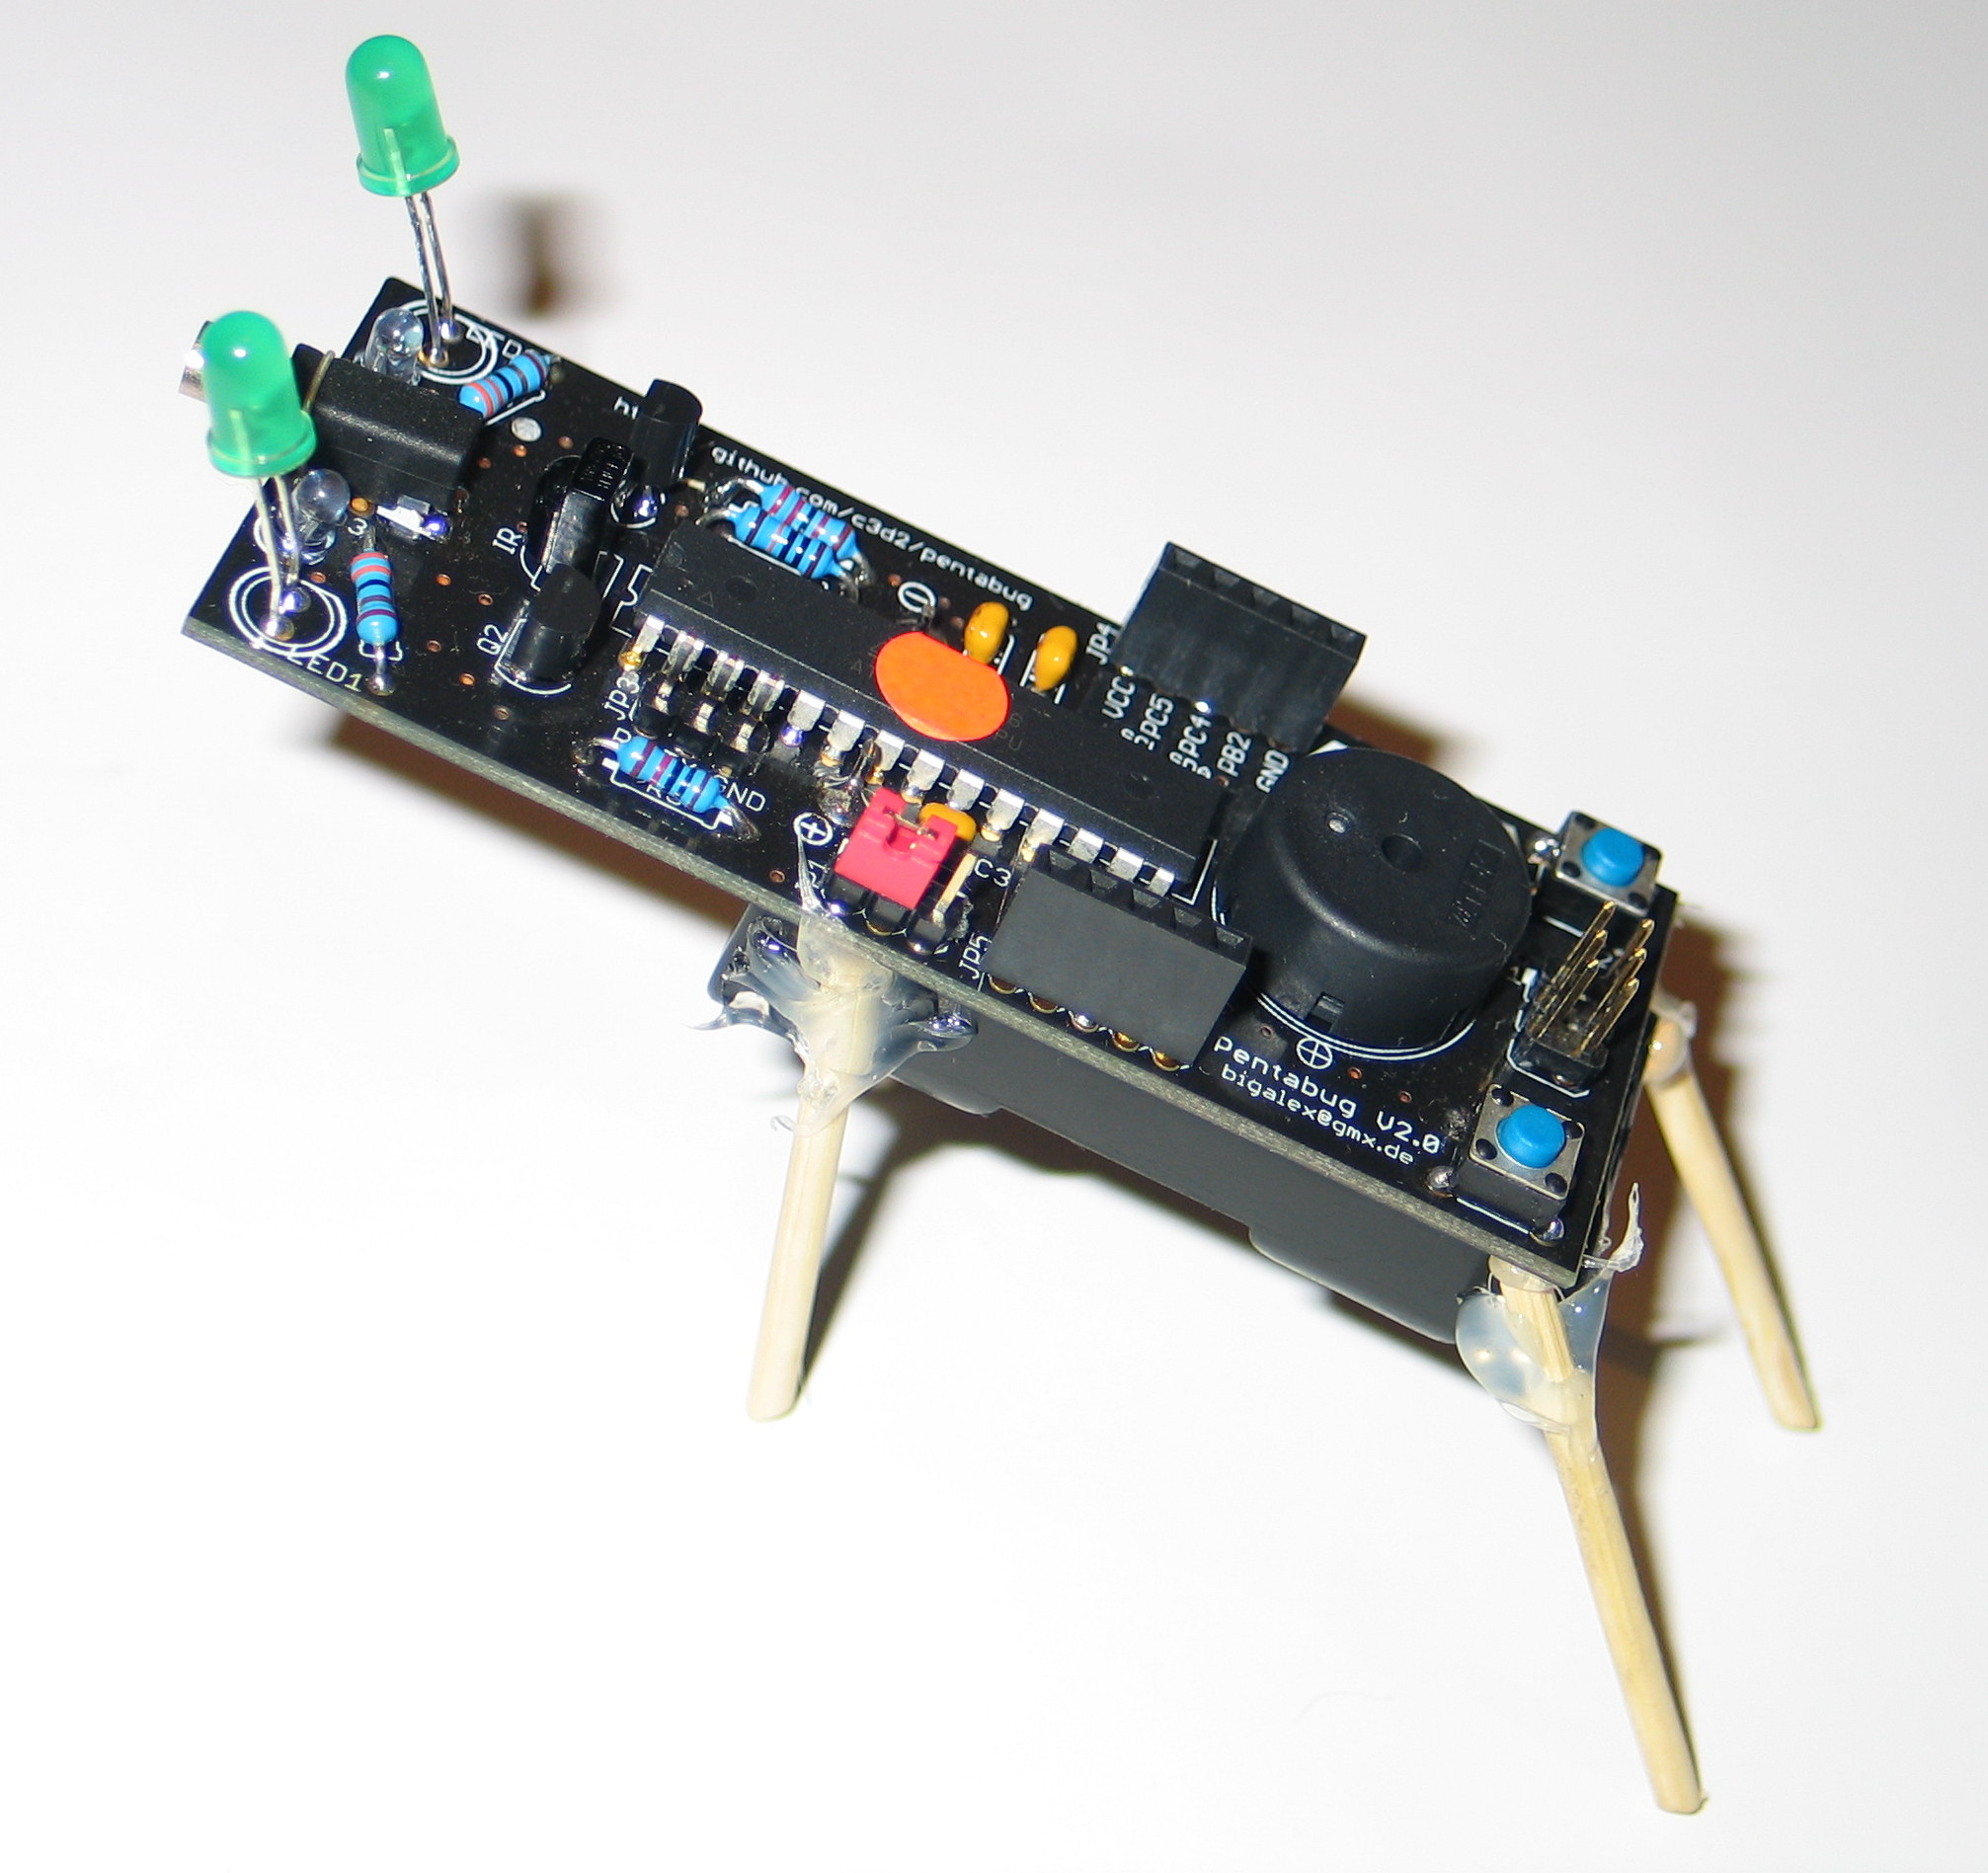
\includegraphics[height=0.5\textheight]{../img/pentabug.jpg}
			}
		\end{center}
	\end{itemize}
\end{frame}

\begin{frame}
	\frametitle{Themen}
	\begin{itemize}
		\item<1-> Überwachung
		\begin{center}
			\only<1>{
				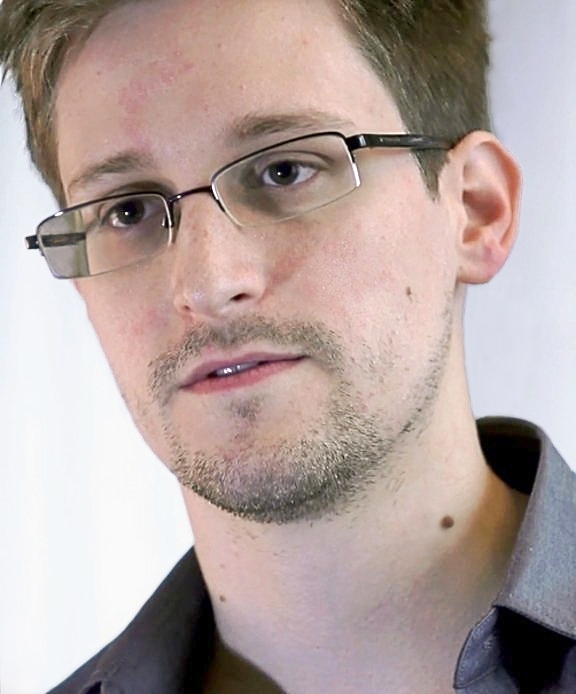
\includegraphics[height=0.7\textheight]{../img/snowden.jpg}
			}
			\only<2>{
				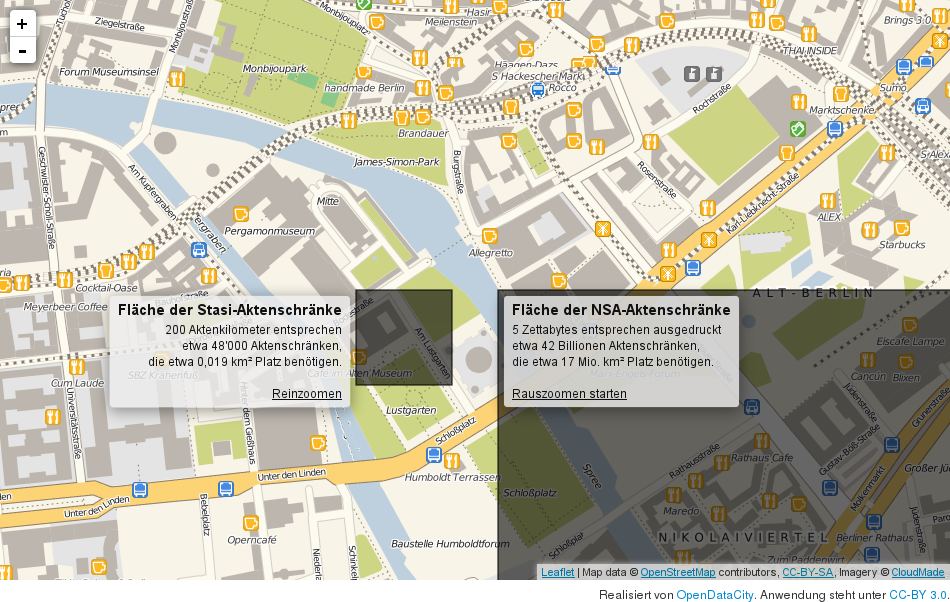
\includegraphics[height=0.7\textheight]{../img/akten1.png}
			}
			\only<3>{
				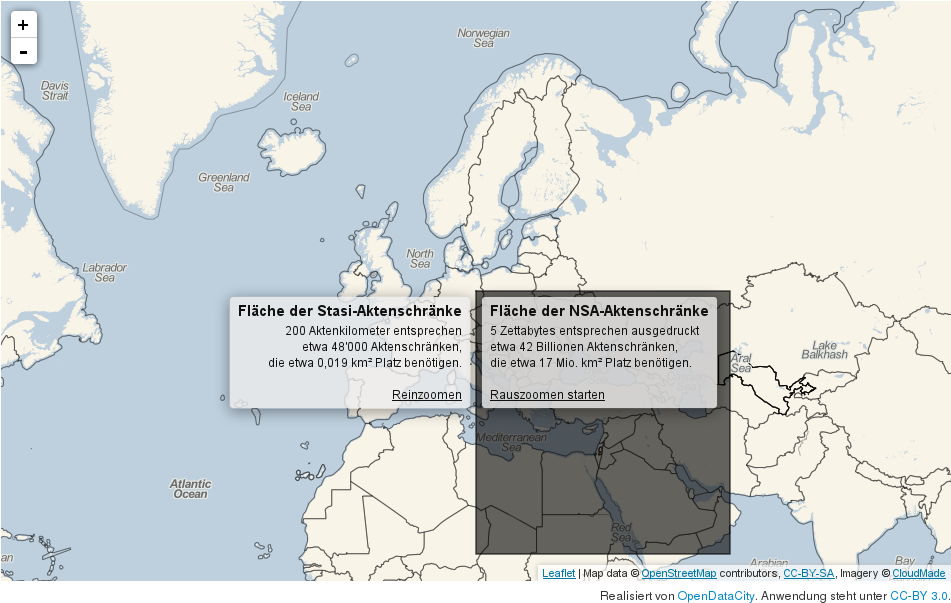
\includegraphics[height=0.7\textheight]{../img/akten2.png}
			}
			\only<4>{
				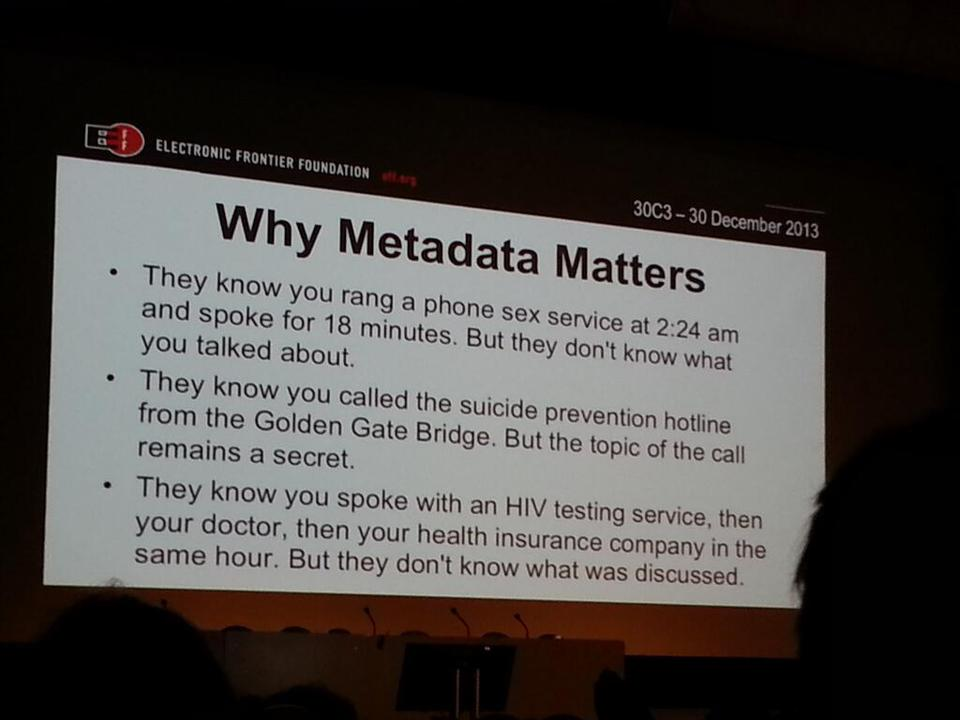
\includegraphics[height=0.7\textheight]{../img/metadata-matters.jpg}
			}	
		\end{center}
	\end{itemize}		
\end{frame}

\begin{frame}
  \frametitle{Themen}
  \begin{itemize}
    \item<1-> Wirtschaft
      \begin{itemize}
        \item<2-> Karstadt
        \item<3-> Amazon
        \item<4-> Ebay
        \item<5-> Facebook
      \end{itemize}
  \end{itemize}
\end{frame}

\begin{frame}
  \frametitle{Themen}
  \begin{figure}
    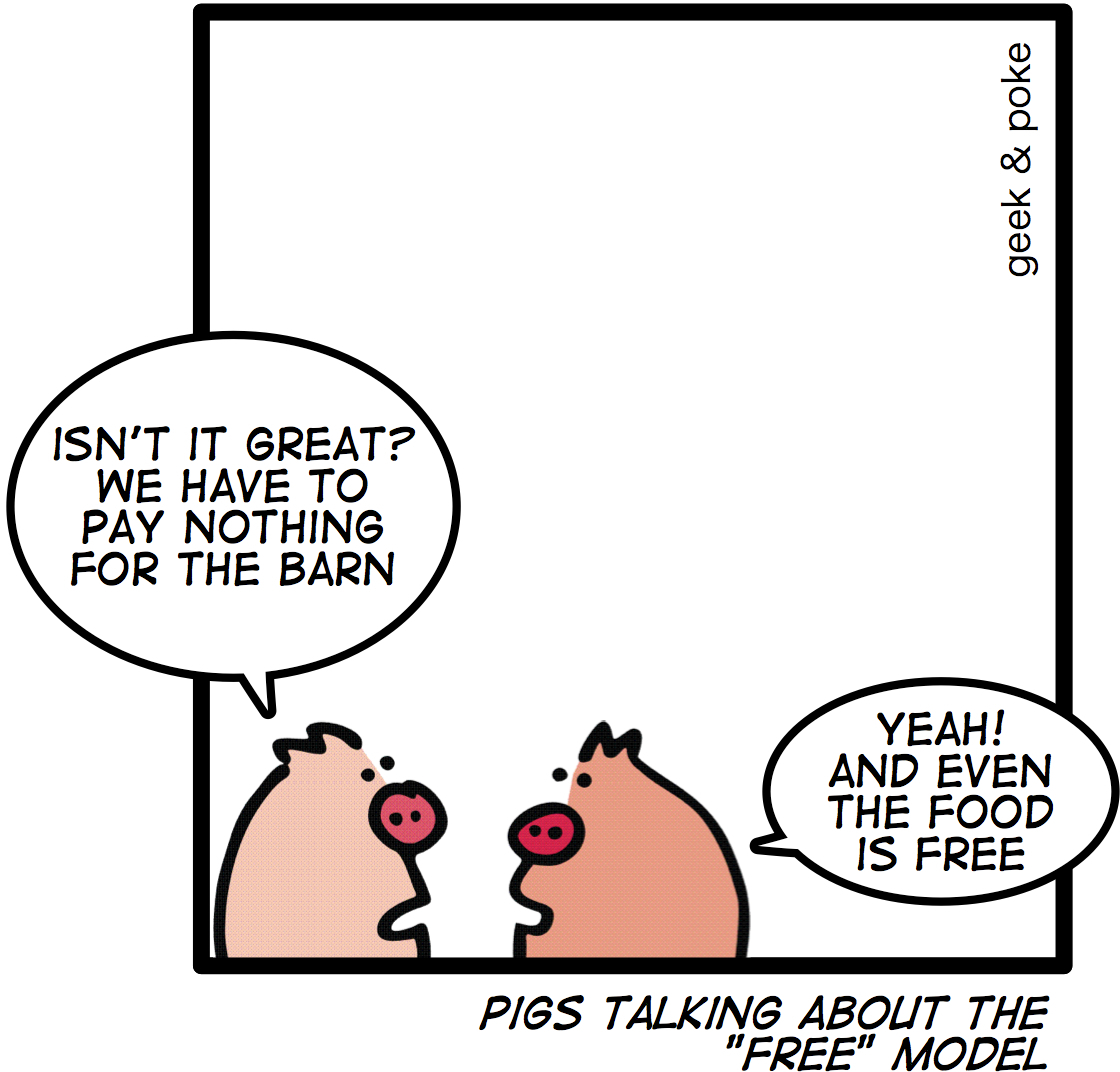
\includegraphics[height=0.7\textheight]{../img/business_pigs.jpg}
  \end{figure}
\end{frame}

\section{Internet}
  \subsection{}

\begin{frame}
	\frametitle{Was ist es für ...}
	\begin{itemize}
		\item<1-> Kinder?
		\begin{center}
			\only<2>{
				
\includegraphics[height=0.7\textheight]{../img/magic_internet.jpg}
			}
		\end{center}
		\item<3-> Jugendliche?
		\begin{center}
			\only<4>{
				
\includegraphics[height=0.7\textheight]{../img/social_networks.jpg}
			}
		\end{center}
		\item<5-> Senioren
		\begin{center}
			\only<6>{
				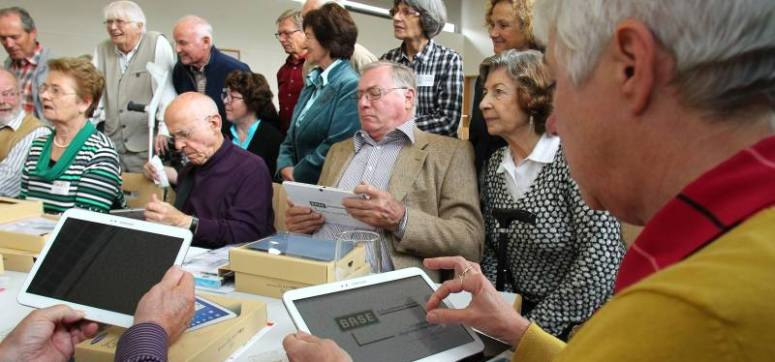
\includegraphics[height=0.5\textheight]{../img/senior.jpg}
			}
		\end{center}
		\item<7-> euch?
		\begin{center}
			\only<7>{
				
\includegraphics[height=0.4\textheight]{../img/frage.jpg}
			}
		\end{center}
	\end{itemize}
\end{frame}
  
\begin{frame}
	\frametitle{Internet}
	\begin{center}
		\only<1>{
			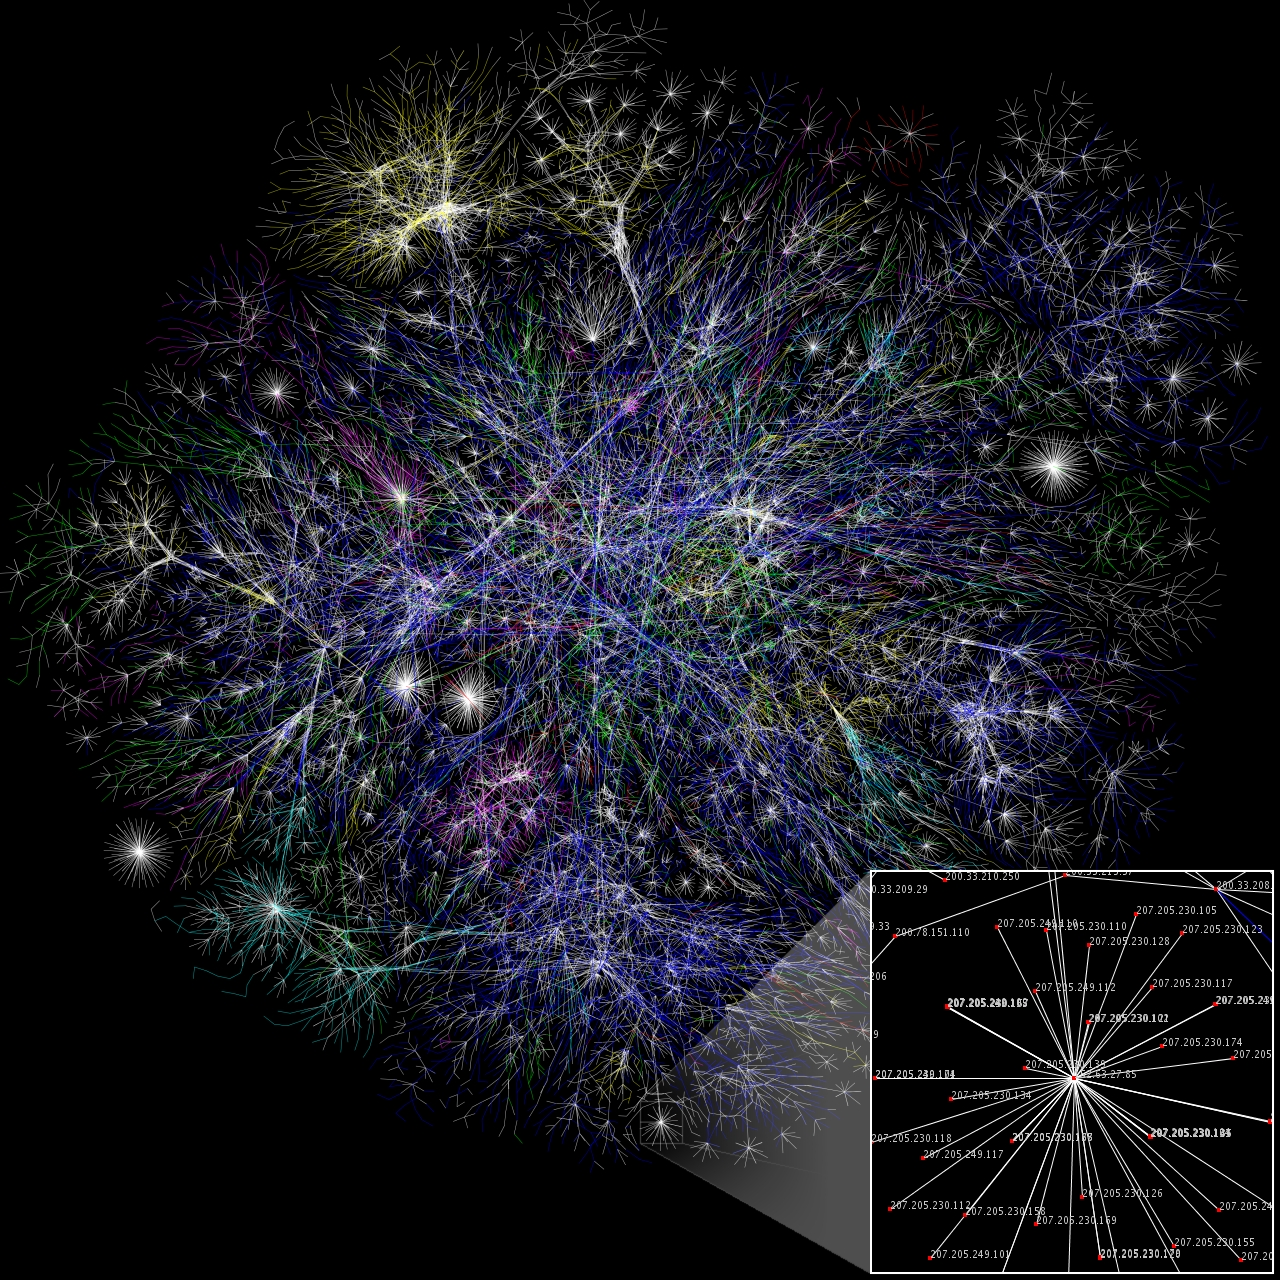
\includegraphics[height=0.7\textheight]{../img/internet_0.jpg}
		}
		\only<2>{
			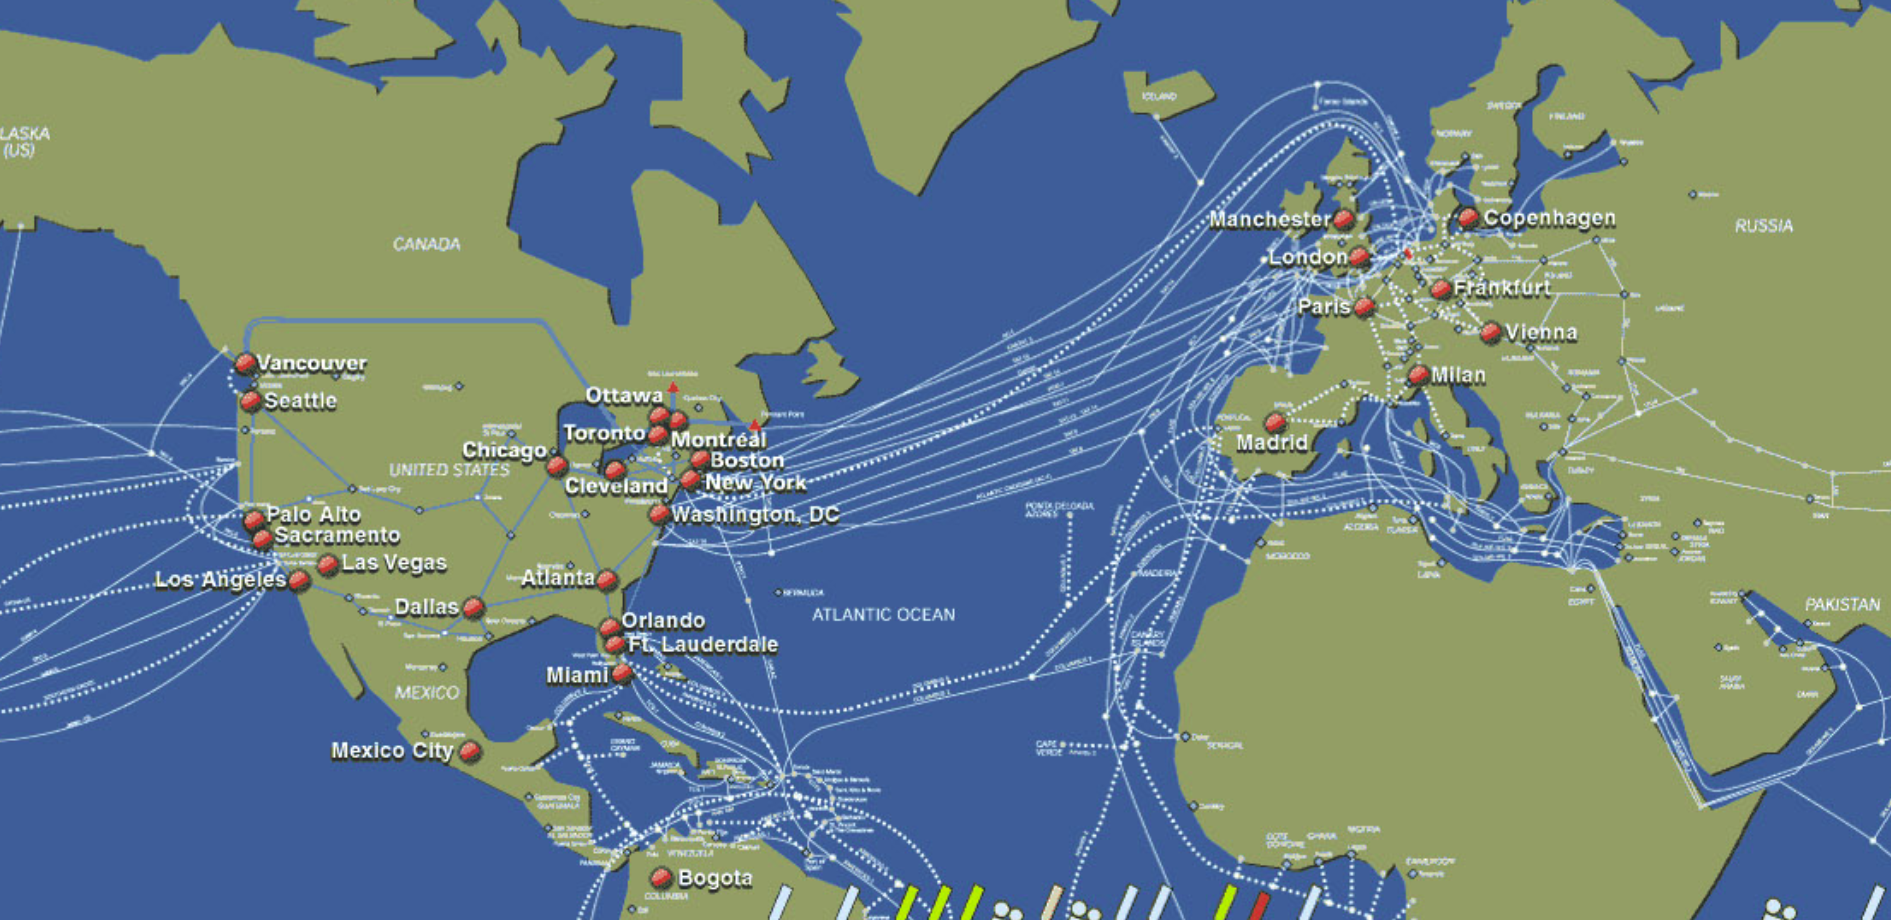
\includegraphics[height=0.6\textheight]{../img/internet_1.png}
		}
		\only<3>{
			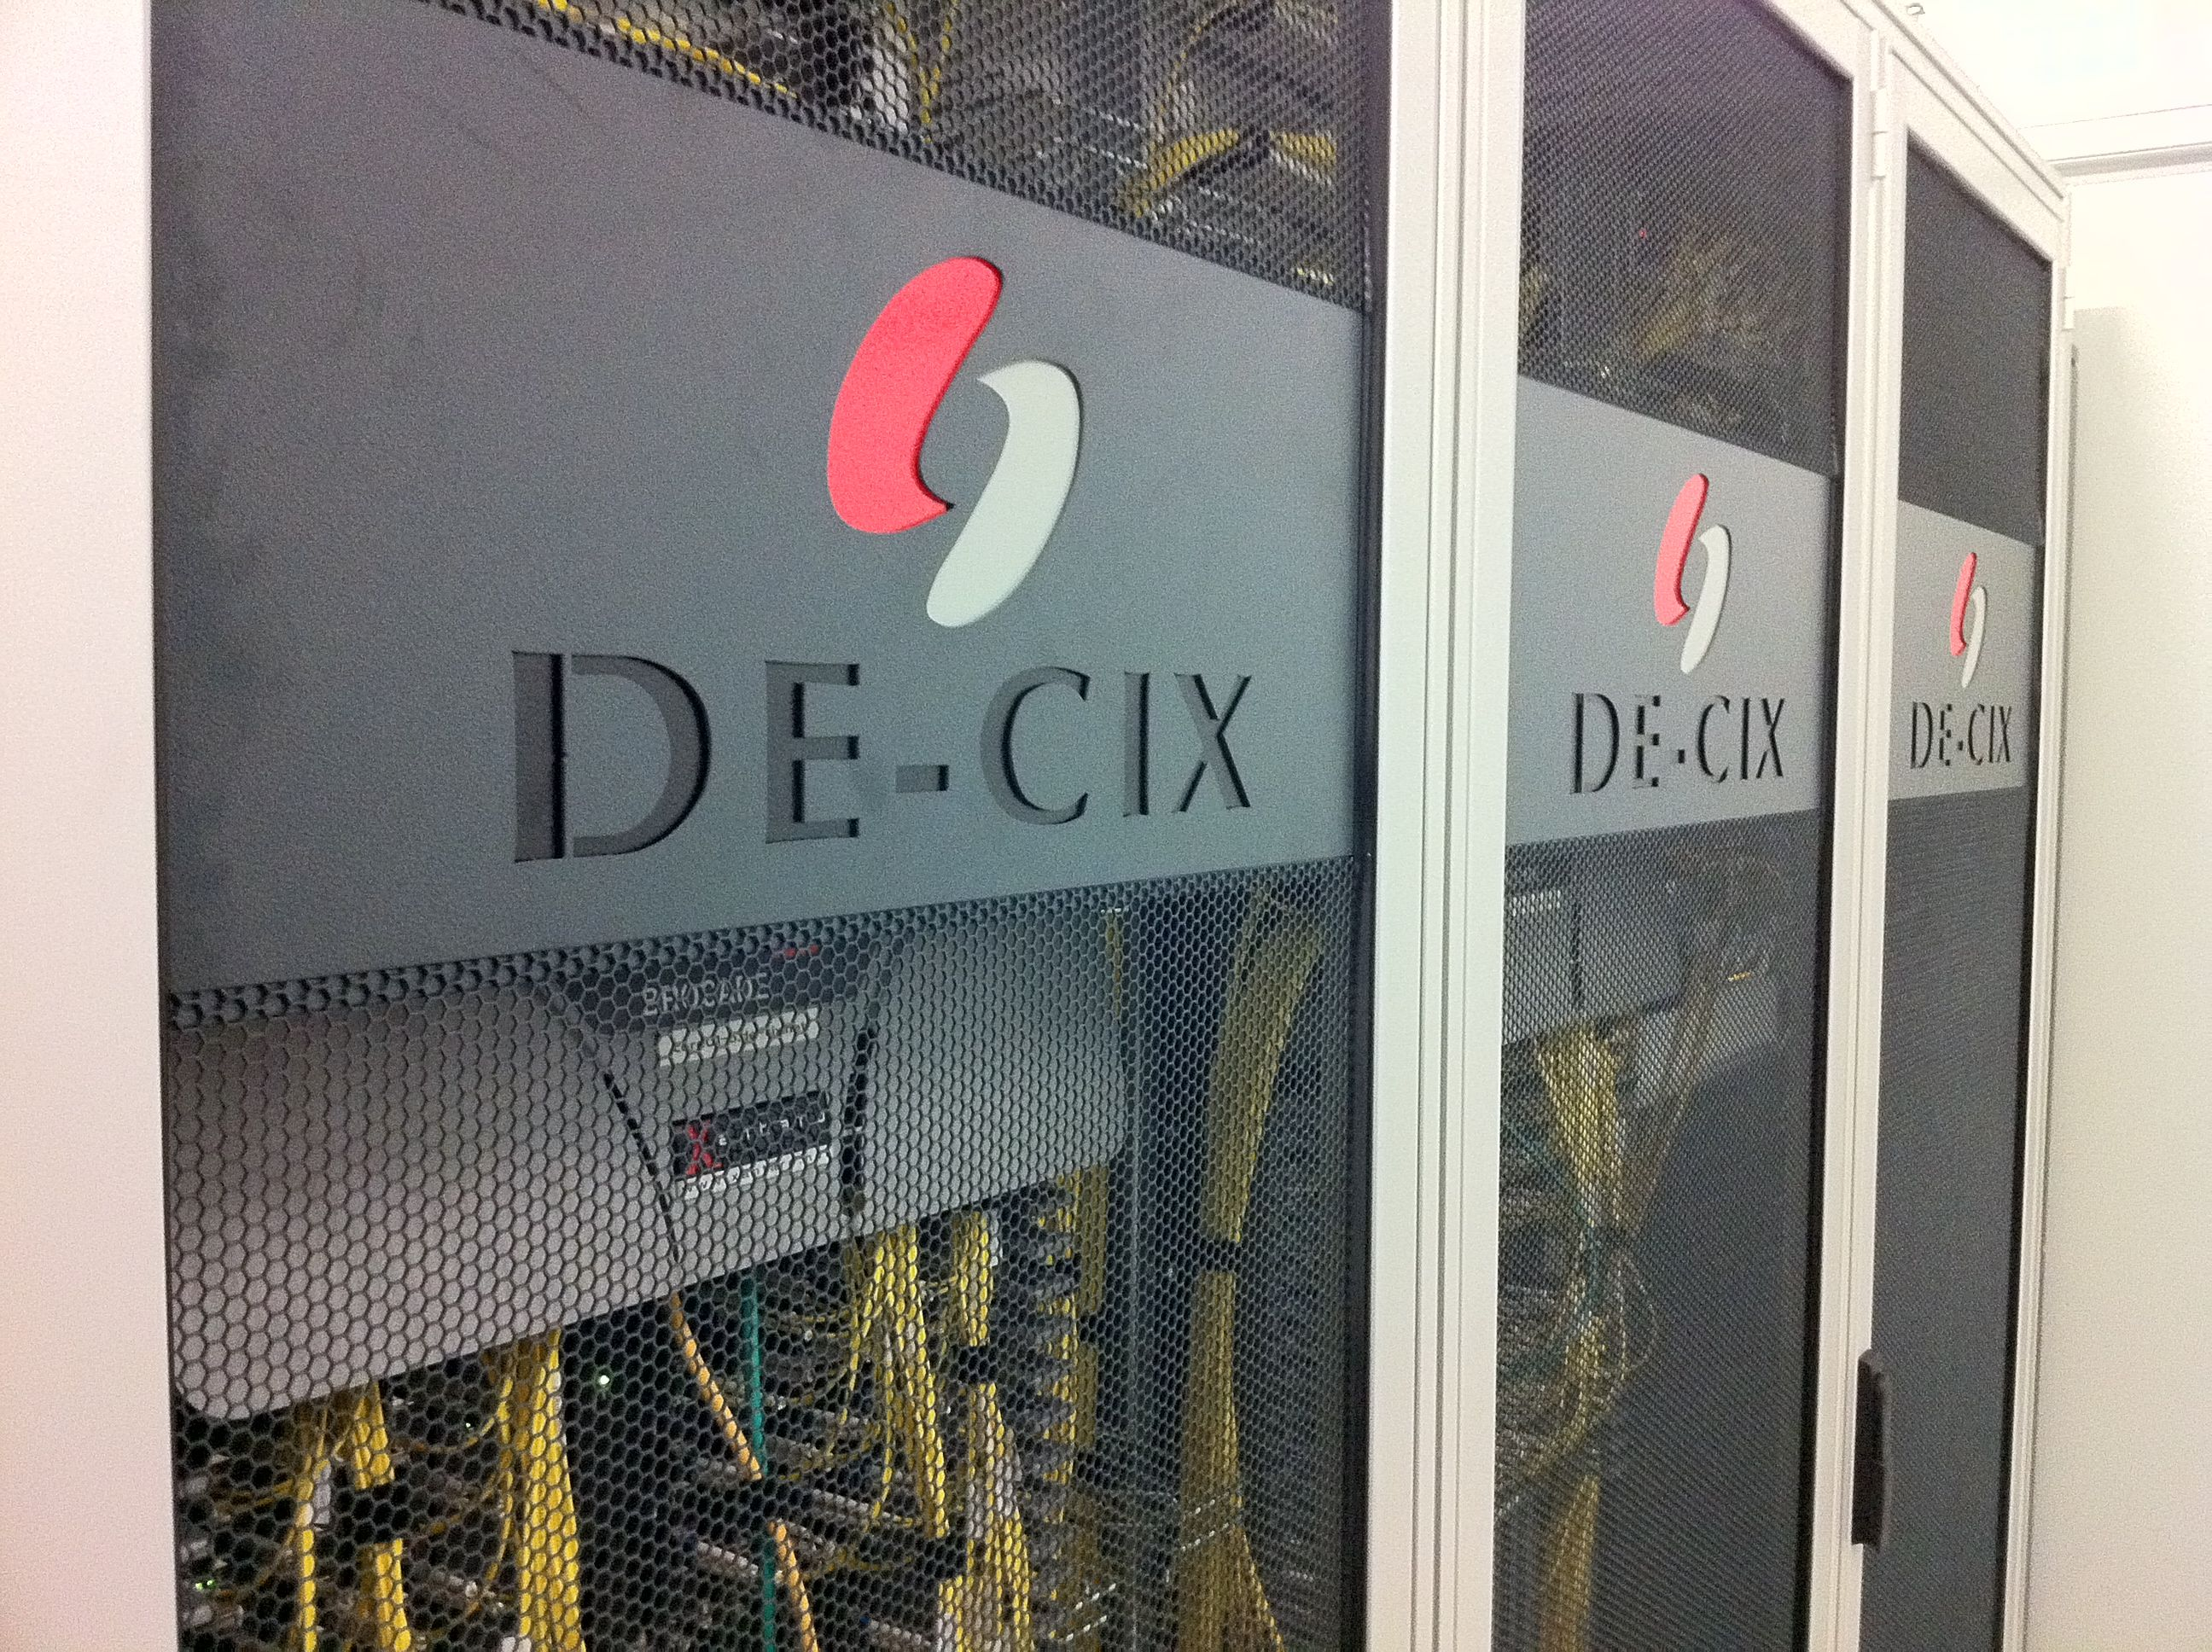
\includegraphics[height=0.6\textheight]{../img/internet_2.jpg}
		}
	\end{center}
\end{frame}

\begin{frame}
	\frametitle{Fazit Internet}
	\begin{itemize}
		\item<1-> dezentral
		\item<2-> senden und empfangen
		\item<3-> neutral
	\end{itemize}
\end{frame}

\section{Zukunft}
  \subsection{}
  
\begin{frame}
	\frametitle{Ein Blick in die Zukunft}
	\begin{itemize}
		\item<1-> SaaS - Software as a Service
		\item<2-> Neuronale Netze
		\item<3-> Überwachung
	\end{itemize}
\end{frame}
  
\begin{frame}
	\frametitle{Schlussworte}
	\begin{itemize}
		\item<1-> Zukunft?
		\item<2-> Lernen, Lernen, Lernen
		\item<3-> Infrastruktur
	\end{itemize}
\end{frame}

\section{Ende}
	\subsection{}

\begin{frame}
	\frametitle{Danksagung}
	\begin{center}
		\textbf{Ein Dank geht an:}
		\begin{itemize}
			\item<1-> die Fakultät für die Einladung
			\item<2-> einen netten Menschen aus der LUG-DD für den W-Lan SSID Sniffer
			\item<3-> an einen netten Menschen für den zweiten Laptop
		\end{itemize}
	\end{center}
\end{frame}
  
\begin{frame}
	\frametitle{Ende}
	\begin{center}
		\textbf{Danke für eure Aufmerksamkeit!} \\
		\textbf{Kontakt: schule@c3d2.de} \\
		\textbf{Fragen?} 
	\end{center}
	\begin{itemize}
		\item<1-> https://c3d2.de/
		\item<2-> https//c3d2.de/schule.html
		\item<4-> https://lists.c3d2.de/  
	\end{itemize}
\end{frame}

\begin{frame}
	\begin{center}
    	
\includegraphics[height=0.5\textheight]{../img/cms-text.png}
    \end{center}
\end{frame}

\end{document}